\newcommand{\U}[1]{\ensuremath{\,\textrm{#1}}}
\newcommand{\tref}{\ensuremath{\textrm{ref}}}
\newcommand{\vthref}{\ensuremath{v_\textrm{thref}}}


\documentclass[fleqn]{report}
\usepackage{fullpage}
\usepackage{amsmath}
\usepackage{amssymb}
\usepackage{bm}
\usepackage{graphicx}


\begin{document}

\title{Inputs and Outputs definition for the linear gyrokinetic database GKDB}

\author{Y. Camenen on behalf of the GKDB working group}

\date{Last update: March 20, 2017}

\maketitle


\chapter{Preamble}

This document summarises the names, conventions and normalisations adopted for the inputs and outputs of the linear gyrokinetic database (GKDB) storing results from $\delta$f, flux-tube gyrokinetic simulations.\\ 

The normalised inputs and outputs are independent of $\rho^*$ consistently with the local approximation and a spectral representation is assumed in the perpendicular plane (i.e. homogeneous turbulence).\\

S.I. units are used everywhere with the exception of temperatures given in eV. This means that $kT$ is noted $T$ as is customary in plasma physics (and possibly confusing).



\chapter{Conventions and normalisations}
\label{chap:normdef}
\section{Cylindrical and flux coordinate systems}
The ITER coordinate convention is adopted for the GKDB. The corresponding index in the COordinate COnventionS system  \cite{Sauter:CPC2013} is COCOS=$11$.
\subsection{Cylindrical coordinate system $(R,\varphi,Z)$}
A right-handed cylindrical coordinate system $(R,\varphi,Z)$, with $R$ the major radius, $Z$ the elevation and $\varphi$ the toroidal angle (increasing when anticlockwise from above) is used to describe the flux surfaces, see Fig.~\ref{fig:coord1}. \\
The magnetic equilibrium is assumed to be axisymmetric and the poloidal contours of the flux surface $\Psi(R,Z)=\Psi_0$, with $\Psi$ the poloidal magnetic flux, are noted $\{R_{\Psi_0},Z_{\Psi_0}\}$.

\begin{figure}[h]
\begin{center}
  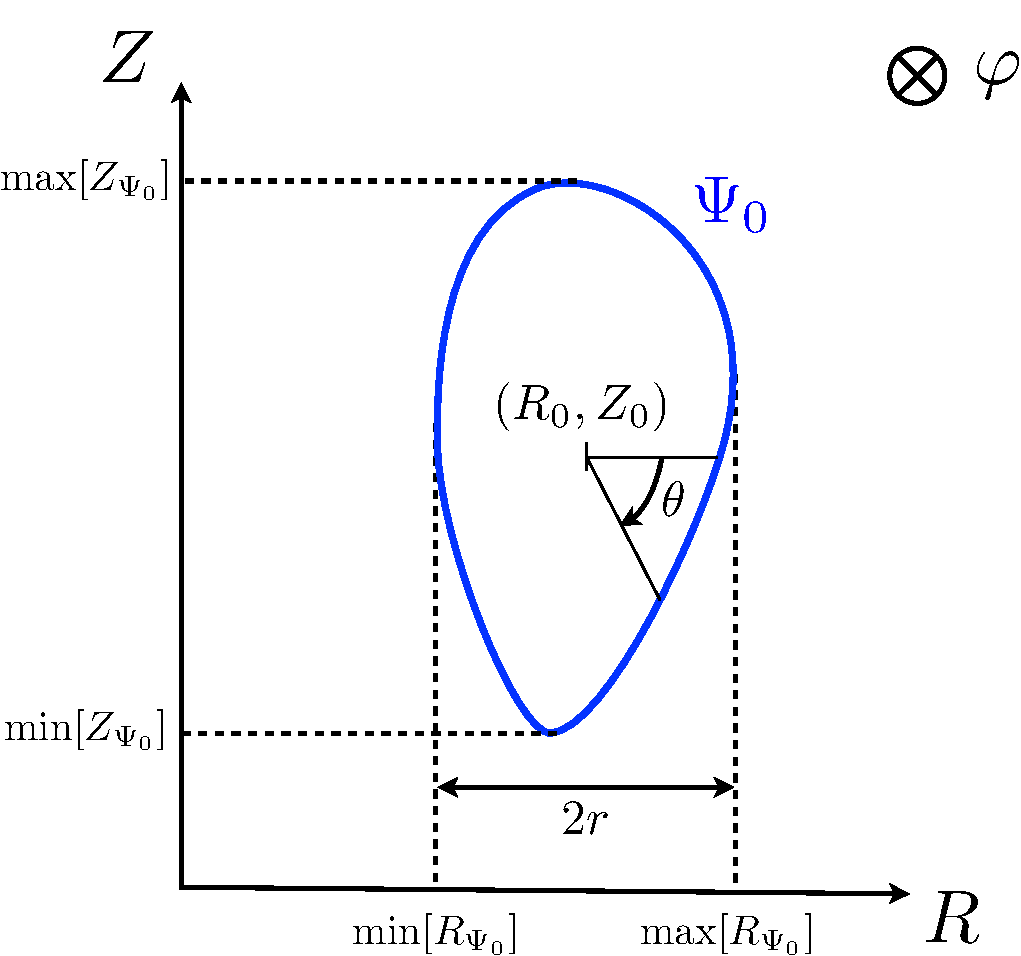
\includegraphics[width=9cm]{COCOS.pdf}\\
  \caption{\label{fig:coord1} Coordinate conventions used in the GKDB (COCOS=11, \cite{Sauter:CPC2013}).}
\end{center}
\end{figure}

\subsection{Flux coordinate system $(r,\theta,\varphi)$}
A right handed flux coordinate system $(r,\theta,\varphi)$ is now introduced.
\subsubsection{Flux surface center}
To start with, a reference point $(R_0,Z_0)$ is defined for the flux surface of interest $\{R_{\Psi_0},Z_{\Psi_0}\}$:
\begin{eqnarray}
 R_0 &=& \frac{1}{2}\left[\max[R_{\Psi_0}] + \min[R_{\Psi_0}]\right]\\
 Z_0 &=& \frac{1}{2}\left[\max[Z_{\Psi_0}] + \min[Z_{\Psi_0}]\right]\\
\end{eqnarray} 
The reference point  $(R_0,Z_0)$ will be used in the following to define the poloidal angle. Note that $(R_0,Z_0)$ is not the position of the magnetic axis, although it can be in some particular cases. 

\subsubsection{Radial coordinate}
The radial coordinate $r$ is defined as 
\begin{equation}
 r = \frac{1}{2}\left[\max[R_{\Psi_0}] - \min[R_{\Psi_0}]\right]
\end{equation}
It has the dimension of a length and is constant on a flux surface, by definition. The radial coordinate of the flux surface $\Psi=\Psi_0$ is noted $r_0$.

\subsubsection{Poloidal angle}
The poloidal angle is defined from the following relationships:
\begin{eqnarray}
 \cos \theta &=& \frac{R_{\Psi_0}-R_0}{\left[ (R_{\Psi_0}-R_0)^2 + (Z_{\Psi_0}-Z_0)^2 \right]^{1/2}}\\
 \sin \theta &=& -\frac{Z_{\Psi_0}-Z_0}{\left[ (R_{\Psi_0}-R_0)^2 + (Z_{\Psi_0}-Z_0)^2 \right]^{1/2}}
\end{eqnarray}
The poloidal angle is zero at the low field side midplane (the midplane is defined with respect to the flux surface $\Psi=\Psi_0$ and corresponds to $Z=Z_0$) and increases clockwise when the tokamak vertical axis is on the left of the flux surface, see Fig.~\ref{fig:coord1}.

\section{Flux surface average}
In a few cases, flux surface averaged quantities will be required. We adopt here the flux surface average definition that arises when taking the integral of a conservation equation over the volume enclosed by a flux surface (i.e. the standard procedure to built 1D transport equations in tokamaks, see for instance \cite{Hinton:RMP1976}).\\
The flux surface average of a quantity $A$ is then given by
\begin{equation}
 <A> = \frac{\int A(\mathbf{x}) \delta(r-r_0) \,\textrm{d}^3{x}}{\int\delta(r-r_0) \,\textrm{d}^3{x}}
\end{equation}
where $r_0$ is the radial coordinate of the flux surface on which the average is being 
performed, $r$ is the value of the radial coordinate at position $\mathbf{x}$, $\delta$ is the Dirac function and the integral is being performed over the whole plasma volume (or entire world, it does not matter).  \\
Noting that the surface element $\textrm{d} S$ on a flux surface is related to the volume element 
$\textrm{d}^3x$ by
\begin{equation}
 \textrm{d}^3x = \textrm{d} S \frac{\textrm{d}r}{|\nabla r|}
\end{equation}
with $r$ an arbitrary flux surface label (taken here to be the radial coordinate defined above), a convenient alternative (and equivalent) expression for the flux surface average is obtained:
\begin{equation} 
 <A> = \frac{1}{V'} \oint A \frac{\textrm{d}S}{|\nabla r|}
\end{equation}
with $V'= \frac{\partial V}{\partial r}$ and $V$ being the volume enclosed by the flux surface labelled by $r$. 

\section{Normalisations}
All quantities in the database (inputs and outputs) are normalised with respect to the reference quantities introduced in this section. Six reference quantities are first introduced (fundamental reference quantities) and then used to built other convenient normalising factors (derived reference quantities).\\
In principle, reference quantities do not need to be specified, as the purpose of the database is to relate normalised inputs to normalised outputs. 
However, if the choice of reference quantities is left arbitrary, the same physical inputs could lead to different normalised inputs in the database depending on the normalisation choice. This is not desirable and the reference quantities are therefore imposed. 

\subsection{Fundamental reference quantities}
The six fundamental reference quantities are:
\begin{itemize}
\item $q_\tref=e=1.6022\times10^{-19}\U{C}$, the positive elementary charge
\item $m_\tref=m_D=3.3445\times10^{-27}\U{kg}$, the Deuterium mass
\item $T_\tref=T_e(r_0,\theta=0)$, the reference electron temperature
\item $n_\tref=n_e(r_0,\theta=0)$, the reference electron density
\item $L_\tref=R_0$, the reference length
\item $B_\tref=B_t(R_0)$, the reference magnetic field (toroidal magnetic field at the flux surface center)
\end{itemize}

\subsection{Derived reference quantities}
For convenience, the following reference quantities are defined:
\begin{itemize}
\item $\vthref=\sqrt{\frac{2T_\tref}{m_\tref}}$, the reference thermal velocity
\item $\rho_\tref = \frac{m_\tref \vthref}{q_\tref B_\tref}$, the reference Larmor radius
\end{itemize}


\chapter{Inputs}
\section{Species}
For each kinetic species $s$, the background distribution function is supposed to be a local Maxwellian. Poloidal asymmetry in the background induced by centrifugal effects is allowed. Poloidally asymmetric quantities are defined at $\theta=0$. Poloidal asymmetry induced by anisotropic temperatures is not included yet, but could be introduced if need be. 
\subsection{Charge}
$$Z_{sN}=\frac{q_s}{q_\tref}$$
\subsection{Mass}
$$m_{sN}=\frac{m_s}{m_\tref}$$
\subsection{Density}
$$n_{sN}=\frac{n_s}{n_\tref}$$
\subsection{Logarithmic density gradient}
$$L_\tref/L_{n_s}=-L_\tref \frac{1}{n_s}\frac{\partial n_s}{\partial r}$$
Positive for peaked profiles. 
\subsection{Temperature}
$$T_{sN}=\frac{T_s}{T_\tref}$$
\subsection{Logarithmic temperature gradient}
$$L_\tref/L_{T_s}=-L_\tref \frac{1}{T_s}\frac{\partial T_s}{\partial r}$$
Positive for peaked profiles.
\subsection{Toroidal velocity}
$$u_{N}=\frac{L_\tref}{\vthref}\omega_{\Phi}$$
Positive for a flow in the direction of $\nabla \varphi$.\\
All species are assumed to have a purely toroidal flow $\mathbf{v}_s=R^2\omega_\Phi\nabla \varphi$ with a common toroidal angular frequency proportional to the background electric field:
$$\omega_{\Phi}=-s_j\frac{1}{|\nabla \Psi|}\frac{\partial \Phi}{\partial r},$$
with $\Phi$ the background electrostatic potential. This assumption is consistent with the ordering used in local gyrokinetic codes, as $\omega_\Phi$ is the lowest order flow in a $\rho_*$ expansion according to neoclassical theory \cite{Hirshman:NF1981}.


\subsection{Toroidal velocity gradient}
$$u'_{sN}=-\frac{L_\tref^2}{\vthref}\frac{\partial \omega_{\varphi,s}}{\partial r}$$
Positive for peaked profiles of a flow in the direction of $\nabla \varphi$.\\
Note that the possibility to have a species dependent toroidal velocity gradient with $\omega_{\varphi,s}\neq \omega_\Phi$ is retained. Strictly speaking, this is inconsistent with the local limit assumption $\rho_*\rightarrow 0$ but can be interesting for the interpretation of the experiments (see the discussion in section II of \cite{Camenen:PoP2016} for more details).

\section{Magnetic equilibrium}
The magnetic equilibrium in the vicinity of the flux surface of interest is specified by the parameters described in this section, given at $r=r_0$.

\subsection{Radial position}
$$r_N=\frac{r_0}{L_\tref}$$

%\subsection{Reference point}
%$$R_{0N} = \frac{R_0}{L_\tref} \qquad \textrm{and} \qquad Z_{0N}=\frac{Z_0}{L_\tref}$$

\subsection{Toroidal field direction}
$$s_b = \textrm{sign}[\mathbf{B}\cdot\nabla\varphi]$$

\subsection{Toroidal current direction}
$$s_j = \textrm{sign}[\mathbf{j}\cdot\nabla\varphi]$$
with $j$ the plasma current density. For the conventions adopted in this document, positive plasma current implies positive poloidal magnetic field.

\subsection{Safety factor}
$$q=\frac{1}{2\pi}\int_0^{2\pi} \frac{\mathbf{B}\cdot\nabla \varphi}{\mathbf{B}\cdot\nabla \theta}\,\textrm{d}\theta$$
Note that $q$ can be positive or negative, its sign depends on the sign of the toroidal plasma current and magnetic field:
$$q = s_b s_j |q|$$

\subsection{Magnetic shear}
$$\hat{s}=\frac{r}{q}\frac{\partial q}{\partial r}$$


\subsection{Pressure gradient}
$$\beta'_N = -\frac{2\mu_0 L_\tref}{B_\tref^2 }\frac{\partial p}{\partial r}$$
with $p$ the total plasma pressure (i.e. the pressure term entering the Grad-Shafranov equation). $\beta'_N$ is a quantity related to the magnetic equilibrium and does not need to be consistent with the gradients ($L_\tref/L_{n_s}$, $L_\tref/L_{T_s}$) specified for the kinetic species. 

\subsection{Plasma shape}
A general description of local magnetic equilibria particularly convenient for gyrokinetic codes was introduced by J. Candy in \cite {Candy:PPCF2009}. It is used in the GKDB with a few minor modifications.
The plasma shape is described by specifying the distance of the constant poloidal flux contours to the reference point $(R_0,Z_0)$  normalised to $L_\tref$:
\begin{equation}
 a_N(r,\theta) = \frac{1}{L_\tref}\sqrt{\left[R_{\Psi}(r,\theta)-R_0\right]^2 + \left[Z_{\Psi}(r,\theta)-Z_0\right]^2}
\end{equation}
To allow regressions in the database the flux surface contours are parametrised as 
\begin{equation}
 a_N(r,\theta) = \sum_{n=0}^{N_{sh}} c_n \cos(n\theta) + s_n \sin(n\theta)
\end{equation}
The specification of the local magnetic equilibrium then requires $4N_{sh}+2$ terms, given at $r=r_0$, where $N_{sh}$ is the degree of the expansion: $\{c_n,s_n,\frac{\partial c_n}{\partial r_N},\frac{\partial s_n}{\partial r_N}\}$. To start with, $N_{sh}$ is set to 8. It should allow to capture most of the plasma shapes but in any case $N_{sh}$ can be increased at a later stage if needed.\\

\section{Modes}
As almost every gyrokinetic codes use a different coordinate system, the Fourier modes needs to be specified in a coordinate free form.\\
To define this coordinate free form, let's first give generic names, $x$ and $y$, to the radial and binormal coordinates used in gyrokinetic codes to describe the turbulence in the plane perpendicular to the magnetic field. The radial coordinate $x$ is assumed to be a flux label (i.e. $\mathbf{B}\cdot \nabla x =0$).
In a spectral representation, perturbed quantities are then written:
\begin{equation}
 f(x,y,\theta) = \sum_{k_x,k_y} \hat{f}(k_x,k_y,\theta)\exp[ik_x x + ik_y y] 
\end{equation}
where $\theta$ is used as the parallel coordinate.
For a given mode, the perpendicular wave vector (in real space) is given by:
\begin{equation}
 k_\perp^2(\theta) = k_x^2 g^{xx} + 2k_xk_y g^{xy} + k_y^2g^{yy}
\end{equation}
with the code dependent metric elements given by $g^{ij}=\nabla i \cdot \nabla j$. All the metric information is on the right hand side of the equation above, the resulting $k_\perp$ does not depend on the specific coordinate choices made in gyrokinetic codes.

\section{Radial mode number}
The normalised coordinate independent radial mode number is defined as
\begin{equation}
 k_{r*}\rho_\tref = k_x \sqrt{g^{xx}(\theta=0)} \rho_\tref
\end{equation}

\section{Binormal mode number}
The normalised coordinate independent binormal mode number is defined as
\begin{equation}
 k_{\theta*}\rho_\tref = k_y \sqrt{g^{yy}(\theta=0)} \rho_\tref
\end{equation}

An alternative convenient specification of the binormal mode number is the effective poloidal mode number normalised to the ion Larmor radius  $nq\rho_\tref/r_0$  \cite{Merlo:PoP2016}. This definition is also coordinate independent and related to a physical quantity. It will not be used here as there is no simple equivalent to specify the radial wave vector.

\section{Electromagnetic effects and collisions}
\subsection{Plasma beta}
The strength of the electromagnetic effects depends on the ratio of the plasma pressure to the magnetic energy and is specified by the dimensionless ratio:
\begin{equation}
\beta_{eN} = 2\mu_0 \frac{n_\tref T_\tref}{B_\tref^2}
\end{equation}
When $\beta_{eN}=0$, the run is electrostatic. 
 
\subsection{Plasma collisionality}
The normalised collision frequency
\begin{equation}
 \nu_{eN} = \frac{q_\tref^2}{16\pi\epsilon_0}\frac{R_\tref n_\tref}{T_\tref^2}
\end{equation}
is used to specify the plasmas collisionality, with $R_\tref$ in $[\textrm{m}]$, $n_\tref$ in $[\textrm{m}^{-3}]$ and $T_\tref$ in $[\textrm{eV}]$. It is assumed that each species collisionality is calculated in the code consistently with the species input parameters (i.e. the normalised species temperature and density are used to calculate the collisionality of each species). This behaviour can be altered by specific collisionality switches described in Sec.~\ref{sec:various}.\\
Sometimes, collisions of electrons on main ions are artificially enhanced by a given factor to mimic the impact of impurity ions. If this was done in the simulation, the enhancement factor is specified with the parameter $Z_\textrm{eff}$.


\section{Various physics} \label{sec:various}
\begin{itemize}
\item adiabatic electrons
\item 
\item electromagnetic switches ($A_\parallel$, $A_\perp$)
\item collisionality switches: pitch angle scattering only or pitch angle and energy scattering? e-i collisions only or e-i, e-e, i-e and i-i? Energy and momentum conserving operator? e-i collisions enhancement by factor Zeff? Test particle operator only and ad-hoc conserving terms or field particle part implemented (as in GS2)? What is the value(s) taken for the Coulomb logarithm? The implementation of collisions is highly code dependent...
\item treatment of the curvature drift (low beta approximation or not)
\end{itemize}

\textit{YC: to be completed...}

\chapter{Outputs}
\section{Mode amplitude}
In linear runs, unstable modes are exponentially growing in time and so are the associated fluxes. 
The exponentially growing outputs are therefore normalised to a dimensionless mode amplitude defined as:
\begin{equation}
 A_f(k_x,k_y)(t) = \sqrt{\int \left[|\hat{\phi}_N(k_x,k_y,\theta)|^2 + |\hat{A}_{\parallel N}(k_x,k_y,\theta)|^2 \right] \,\textrm{d}\theta}
\end{equation}
with the Fourrier components of the electrostatic potential and vector potential normalised as follows:
\begin{equation}
  \hat{\phi}_N = \frac{q_\tref}{T_\tref} \hat{\phi} \qquad \qquad 
\textrm{and} \qquad \qquad \hat{A}_{\parallel N}=\frac{1}{B_\tref \rho_\tref} \hat{A}_\parallel
\end{equation}


\section{Mode growth rate and frequency}
The normalisations of the mode growth rate $\gamma$ and frequency $\omega_r$ are:
\begin{equation}
 \gamma_N(k_x,k_y) = \gamma(k_x,k_y) \frac{L_\tref}{v_\textrm{thref}} \qquad \qquad \textrm{and} \qquad \qquad \omega_{rN}(k_x,k_y) = \omega_r(k_x,k_y) \frac{L_\tref}{v_\textrm{thref}}
\end{equation}
By convention, unstable modes have a positive growth rate and modes propagating in the ion diamagnetic drift direction have a positive frequency (and therefore a negative frequency when they are propagating in the electron diamagnetic drift direction).

\section{Parallel mode structure}
\subsection{Perturbed electrostatic potential}
\subsection{Perturbed parallel vector potential (magnetic field flutter)}
\subsection{Perturbed parallel magnetic field (magnetic field compression)}
\textit{YC: to do, find an appropriate basis to expand the parallel mode structure}

\section{Fluxes}
\subsection{Definition}
For each species, the flux-surface averaged contravariant radial component of the particle flux, energy flux and toroidal angular momentum flux are given by:
\begin{eqnarray}
 \Gamma_s &=& \left<\int f_s \mathbf{v}_\mathbf{E} \cdot \nabla r\,\textrm{d}\mathbf{v}\right> 
+ \left<\int f_s \mathbf{v}_{\mathbf{B}_\perp} \cdot \nabla r\,\textrm{d}\mathbf{v}\right> \\
      Q_s &=& \left<\int \frac{1}{2}m_sv^2 f_s \mathbf{v}_\mathbf{E} \cdot \nabla r\,\textrm{d}\mathbf{v}\right> 
+ \left<\int \frac{1}{2}m_sv^2 f_s \mathbf{v}_{\mathbf{B}_\perp} \cdot \nabla r\,\textrm{d}\mathbf{v}\right> \\
  \Pi_s   &=& \left<\int m_s R \frac{B_t}{B}v_\parallel f_s \mathbf{v}_\mathbf{E} \cdot \nabla r\,\textrm{d}\mathbf{v}\right> 
+ \left<\int m_s R \frac{B_t}{B}v_\parallel f_s \mathbf{v}_{\mathbf{B}_\perp} \cdot \nabla r\,\textrm{d}\mathbf{v}\right>
% + <\int \alpha_i f_s \mathbf{v}_{\nabla B_\parallel} \cdot \nabla r\,\textrm{d}\mathbf{v}>
% YC: possible to add compressional effects later on, but then the expression must take into account the difference between guiding centers and particles (note to self: see document by G. Szepesi)
\end{eqnarray}
where $f_s$ is the perturbed guiding center distribution function of species $s$ and the two terms on the right hand side correspond to the fluxes induced by the electrostatic and magnetic flutter drifts:
\begin{equation}
 \mathbf{v}_\mathbf{E} = \frac{\mathbf{b}\times \nabla \phi}{B} \qquad \qquad \textrm{and } \qquad \qquad
 \mathbf{v}_{\mathbf{B}_\perp} = -v_\parallel \frac{\mathbf{b}\times \nabla A_{\parallel}}{B} 
%  \mathbf{v}_{\nabla B_\parallel} = \frac{\mu}{Ze} \frac{\mathbf{b}\times \nabla B_{1\parallel}}{B}
\end{equation}
with $\phi$ and $A_{1\parallel}$ the gyro-averaged perturbed electrostatic potential and  parallel vector potential, respectively.
Note that the toroidal angular momentum only includes the toroidal projection of the parallel momentum, but rigourously speaking one should also include the toroidal projection of the perpendicular momentum (\textit{YC: to be added, but it is almost always negligible...}). 
\subsection{Coordinate free form}
As the contravariant radial component of the fluxes is coordinate dependent, the particle, energy and toroidal angular momentum transfer rates accross the flux surface $r_0$, are preferred to the fluxes to characterise the level of transport: $T_s^p=\Gamma_s \mathcal{V}'$, $T_s^m=\Pi_s\mathcal{V}'$ and $T_s^e=Q_s\mathcal{V}'$, where $\mathcal{V}'=\partial\mathcal{V}/\partial r$ with  $\mathcal{V}$ the volume enclosed by the flux surface $r=r_0$. 

\subsection{Normalisation}
The transfer rates are given for each Fourier mode. They are normalised to the corresponding (linear) mode amplitude and made dimensionless as follows:
\begin{eqnarray}
 T^p_{Ns}(k_x,k_y) &=& \frac{1}{A_f}\frac{\Gamma_s(k_x,k_y)\mathcal{V}'}{n_\tref v_\textrm{thref} L_\tref^2}\\
 T^m_{Ns}(k_x,k_y) &=& \frac{1}{A_f}\frac{\Pi_s(k_x,k_y)\mathcal{V}'}{n_\tref v_\textrm{thref} L_\tref^2}\\
 T^e_{Ns}(k_x,k_y) &=& \frac{1}{A_f}\frac{Q_s(k_x,k_y)\mathcal{V}'}{n_\tref v_\textrm{thref} L_\tref^2}
\end{eqnarray}
In addition, the electrostatic and magnetic flutter parts are given separately (i.e. $T_{Ns}=T_{Ns,\phi}+T_{Ns,A_\parallel}$) for each transfer rate. 




\chapter{Meta-data}

\chapter{Summary tables}

\textit{TO DO: add summary tables for normalising quantities, inputs and outputs with hyperlinks to the detailed definitions for convenience}

\chapter{Test cases}

\section{Test 1}
A simple electrostatic test case close to the GA standard case with kinetic electrons.
\subsection{Species}
\begin{tabular}{c c c c c c c c c c}
\hline
Species & $Z_{sN}$ & $m_{sN}$ & $n_{sN}$ & $T_{sN}$ & $L_\tref/L_{n_s}$ & $L_\tref/L_{T_s}$ & $u_{sN}$ & $u'_{sN}$ \\ [0.5ex]
\hline
e & -1 & $2.7232\times10^{-4}$ & 1 & 1 & 3 & 9 & 0 & 0 \\ [0.5ex]
\hline 
D &  1 & 1 & 1 & 1 & 3 & 9 & 0 & 0 \\ [0.5ex]
\hline
\end{tabular}

\subsection{Magnetic equilibrium}
\begin{tabular}{c c c c c c c}
\hline
$r_N$ & $R_{0N}$ & $q$ & $\hat{s}$ & $s_b$ & $s_j$ & $\beta'_N$ \\ [0.5ex]
\hline
0.16 & 1 & 2 & 1 & 1 & 1 & 0 \\
\hline
\end{tabular}\\
\begin{tabular}{c c c c c c c c c c c c c}
\hline
$\alpha_0$ & $\alpha_1$ & $\alpha_2$ & $\alpha_3$ & $\alpha_4$ & $\alpha_5$ & $\alpha_6$ 
& $\beta_1$ & $\beta_2$ & $\beta_3$ & $\beta_4$ & $\beta_5$ & $\beta_6$   \\ [0.5ex]
\hline
 0.16 & 0 & 0 & 0 & 0 & 0 & 0 & 0 & 0 & 0 & 0 & 0 & 0 \\
\hline
\end{tabular}\\
\begin{tabular}{c c c c c c c c c c c c c}
\hline
$\alpha'_0$ & $\alpha'_1$ & $\alpha'_2$ & $\alpha'_3$ & $\alpha'_4$ & $\alpha'_5$ & $\alpha'_6$ 
& $\beta'_1$ & $\beta'_2$ & $\beta'_3$ & $\beta'_4$ & $\beta'_5$ & $\beta'_6$   \\ [0.5ex]
\hline
1.0 & 0 & 0 & 0 & 0 & 0  & 0 & 0 & 0 & 0  & 0 & 0 & 0 \\
\hline
\end{tabular}

\subsection{Modes}
\begin{tabular}{c c c c c}
\hline
$k_{\theta*}\rho_\tref$ & 0.2 & 0.4 & 0.6 & 0.8 \\ [0.5ex]
\hline
$k_{r*}\rho_\tref$ & -0.2 & 0  & 0.2  &  \\ [0.5ex]
\hline
\end{tabular}

\subsection{Collisionality and beta}
\begin{tabular}{c c}
\hline
 $\beta_{eN}$ & $\nu_N$ \\ [0.5ex]
\hline
0 & 0 \\ [0.5ex]
\hline
\end{tabular}

\section{Test 2}
Same with shaping.

\subsection{Species}
\begin{tabular}{c c c c c c c c c c}
\hline
Species & $Z_{sN}$ & $m_{sN}$ & $n_{sN}$ & $T_{sN}$ & $L_\tref/L_{n_s}$ & $L_\tref/L_{T_s}$ & $u_{sN}$ & $u'_{sN}$ \\ [0.5ex]
\hline
e & -1 & $2.7232\times10^{-4}$ & 1 & 1 & 3 & 9 & 0 & 0 \\ [0.5ex]
\hline 
D &  1 & 1 & 1 & 1 & 3 & 9 & 0 & 0 \\ [0.5ex]
\hline
\end{tabular}

\subsection{Magnetic equilibrium}
\begin{tabular}{c c c c c c c}
\hline
$r_N$ & $R_{0N}$ & $q$ & $\hat{s}$ & $s_b$ & $s_j$ & $\beta'_N$ \\ [0.5ex]
\hline
0.5 & 1 & 2 & 1 & 1 & 1 & 0.03 \\
\hline
\end{tabular}\\
\begin{tabular}{c c c c c c c c c c c c c}
\hline
$\alpha_0$ & $\alpha_1$ & $\alpha_2$ & $\alpha_3$ & $\alpha_4$ & $\alpha_5$ & $\alpha_6$ 
& $\beta_1$ & $\beta_2$ & $\beta_3$ & $\beta_4$ & $\beta_5$ & $\beta_6$   \\ [0.5ex]
\hline
 0.5831 & -0.0242 & -0.0987 & 0.0321 & 0.0174 & -0.0107 & -0.0020 & 0 & 0 & 0 & 0 & 0 & 0 \\
\hline
\end{tabular}\\
\begin{tabular}{c c c c c c c c c c c c c}
\hline
$\alpha'_0$ & $\alpha'_1$ & $\alpha'_2$ & $\alpha'_3$ & $\alpha'_4$ & $\alpha'_5$ & $\alpha'_6$ 
& $\beta'_1$ & $\beta'_2$ & $\beta'_3$ & $\beta'_4$ & $\beta'_5$ & $\beta'_6$   \\ [0.5ex]
\hline
1.2898 & -0.3984 & -0.3892 & 0.2734 & 0.1136 & -0.1085  & -0.0097 & 0.2892 & 0.0195 & -0.0417  & 0.0153 & 0.0140 & -0.0065 \\
\hline
\end{tabular}

\subsection{Modes}
\begin{tabular}{c c c c c}
\hline
$k_{\theta*}\rho_\tref$ & 0.2 & 0.4 & 0.6 & 0.8 \\ [0.5ex]
\hline
$k_{r*}\rho_\tref$ & -0.2 & 0  & 0.2  &  \\ [0.5ex]
\hline
\end{tabular}

\subsection{Collisionality and beta}
\begin{tabular}{c c}
\hline
 $\beta_{eN}$ & $\nu_N$ \\ [0.5ex]
\hline
0 & 0 \\ [0.5ex]
\hline
\end{tabular}

\bibliographystyle{unsrt}
\bibliography{IOGKDB}

\end{document}



